\documentclass[runningheads,a4paper]{llncs}
\usepackage[T1]{fontenc}
\usepackage{newtxtext}
\usepackage[varvw]{newtxmath}
\usepackage{graphicx}
\usepackage{amsmath}
\usepackage{booktabs}
\usepackage{tikz}
\usetikzlibrary{arrows.meta}
\usepackage[hidelinks]{hyperref}
\hypersetup{pdftitle={X-Fusion: Tri-Modal Transformer Fusion for Multi-Label Chest X-ray Analysis},pdfauthor={},pdfsubject={Anonymous review manuscript},pdfkeywords={multimodal learning, chest radiography}}
\begin{document}
\title{X-Fusion: Tri-Modal Transformer Fusion for Multi-Label Chest X-ray Analysis}
\titlerunning{X-Fusion for Multi-Label Chest X-ray Analysis}
\author{Anonymous Authors}
\authorrunning{Anonymous Authors}
\institute{Anonymous Institution}
\maketitle
\begin{abstract}
We present X-Fusion, a tri-modal Transformer prototype for multi-label chest radiograph analysis. The system combines BiomedCLIP image representations, CXR-BERT clinical-text embeddings, and six structured patient attributes in a shared 512-dimensional space. A two-layer, eight-head Transformer integrates the modalities through a learned classification token and predicts fourteen thoracic findings. Training combines Asymmetric Loss with image--text contrastive alignment, while a web interface presents predictions alongside visual attention and metadata-attribution views. We document the implementation and examine available artifacts from a patient-disjoint subset of 31,630 ChestX-ray14 images. We additionally train independent-input reference models using only image pixels and recorded age and sex, with hyperparameters selected on validation patients and evaluation on 7,100 test-list images. Recomputed metrics indicate that the existing pipeline fits its evaluation inputs closely. Crucially, the notes and several physiological measurements were generated using reference labels; these scores therefore describe the implemented pipeline rather than independent diagnostic accuracy. The study contributes a compact software integration, a reproducible independent-input baseline experiment, and an explicit analysis of the remaining evidence needed to validate tri-modal fusion.
\keywords{Chest radiography \and Multimodal learning \and Transformer fusion \and Evaluation leakage}
\end{abstract}
\section{Introduction}

Chest radiography is widely used for evaluating thoracic abnormalities. A single image may exhibit several coexisting findings, making multi-label classification more appropriate than mutually exclusive disease prediction. NIH ChestX-ray14 provides a benchmark for this setting \cite{wang2017,nihdataset}. Visual patterns can be ambiguous without clinical context. Patient history and physiological measurements may offer complementary information when these inputs are collected independently of the reference diagnosis.

X-Fusion integrates three information streams comprising a radiograph, a clinical note, and six structured patient attributes. Pretrained BiomedCLIP and CXR-BERT representations are projected into a common feature space and combined with an MLP-based metadata representation using Transformer self-attention. The framework predicts fourteen labels and exposes attention and metadata attribution views through a web interface. The contributions are an implemented four-token integration of established pretrained encoders and losses, an inference interface with distinct visual and metadata views, and a controlled reference experiment with independently observed image and demographic predictors. We do not claim invention of the underlying attention, loss, or attribution methods. We also analyze saved training and prediction records to characterize the prototype under its documented evaluation setup.



The original tri-modal experiment uses an auxiliary-input generator that conditions clinical notes and selected vital signs on reference labels. We account for this dependency when interpreting its saved predictions; patient-disjoint splitting alone cannot eliminate it. The new reference experiment excludes those generated inputs.

\section{Related Work}

Wang et al. introduced the NIH chest radiograph benchmark \cite{wang2017}. CheXpert later addressed uncertain labels and expert comparison \cite{irvin2019}. Vision Transformers model long-range relationships through attention \cite{dosovitskiy2021,vaswani2017}. BiomedCLIP learns biomedical visual representations from image and text pairs \cite{biomedclip2023}, while CXR-BERT specializes language representations for radiology \cite{cxrbert2022}. DAViT explores domain-adapted Transformer modeling for pneumonia detection \cite{davit2025}, a distinct single-disease setting. Asymmetric Loss addresses class imbalance \cite{ridnik2021}. InfoNCE supports representation alignment \cite{oord2018}, while SHAP provides feature attribution \cite{lundberg2017}. Attention visualization alone should not be interpreted as validated disease localization \cite{chefer2021}.

\section{Proposed Architecture and Methodology}

\subsection{Modality-Specific Encoders}

For an RGB radiograph $I$, a tokenized note $T$, and ordered metadata vector $m\in\mathbb{R}^{6}$, the encoders produce

\begin{align}
z_v &= f_v(I)\in\mathbb{R}^{512},
\label{eq:vision}\\
z_t &= W_t h_t(T)+b_t\in\mathbb{R}^{512},
\label{eq:text}\\
u &= \operatorname{Dropout}_{0.1}
(\operatorname{GELU}(W_1m+b_1)),
\label{eq:meta1}\\
z_m &= \operatorname{GELU}(W_2u+b_2)
\in\mathbb{R}^{512}.
\label{eq:meta2}
\end{align}

BiomedCLIP supplies pooled image features. The first CXR-BERT output token is projected from 768 to 512 dimensions, with notes limited to 256 tokens. The metadata encoder maps age, sex, temperature, heart rate, respiratory rate, and oxygen saturation through a 128-unit hidden layer. The weight matrices have dimensions $W_1\in\mathbb{R}^{128\times6}$ and $W_2\in\mathbb{R}^{512\times128}$.

\subsection{Transformer Fusion}

The learned classification token and three modality vectors form

\begin{equation}
S_0=[e_{\mathrm{CLS}};z_v;z_t;z_m]
\in\mathbb{R}^{4\times512}.
\end{equation}

Two Transformer encoder layers use eight attention heads and a feed-forward width of 2048. Attention is computed as

\begin{equation}
\operatorname{Attention}(Q,K,V)
=\operatorname{softmax}\!\left(\frac{QK^{\top}}{\sqrt{d_k}}\right)V.
\end{equation}

Here $Q$, $K$, and $V$ are query, key, and value matrices, and softmax is applied row-wise. The fusion encoder has eight heads, so each key has width $d_k=512/8=64$. The fused CLS vector is classified with dropout probability 0.3.

\begin{equation}
\begin{aligned}
h &= \operatorname{Transformer}(S_0)_{\mathrm{CLS}},\\
p_k &= \sigma\!\left(
\left[W_c\operatorname{Dropout}_{0.3}(h)+b_c\right]_k
\right).
\end{aligned}
\end{equation}

Here $W_c\in\mathbb{R}^{14\times512}$ and $k=1,\ldots,14$. The findings are Atelectasis, Cardiomegaly, Effusion, Infiltration, Mass, Nodule, Pneumonia, Pneumothorax, Consolidation, Edema, Emphysema, Fibrosis, Pleural Thickening, and Hernia.

\begin{figure}[t]
\centering
\resizebox{\linewidth}{!}{% Editable vector architecture diagram for X-Fusion; TikZ required.
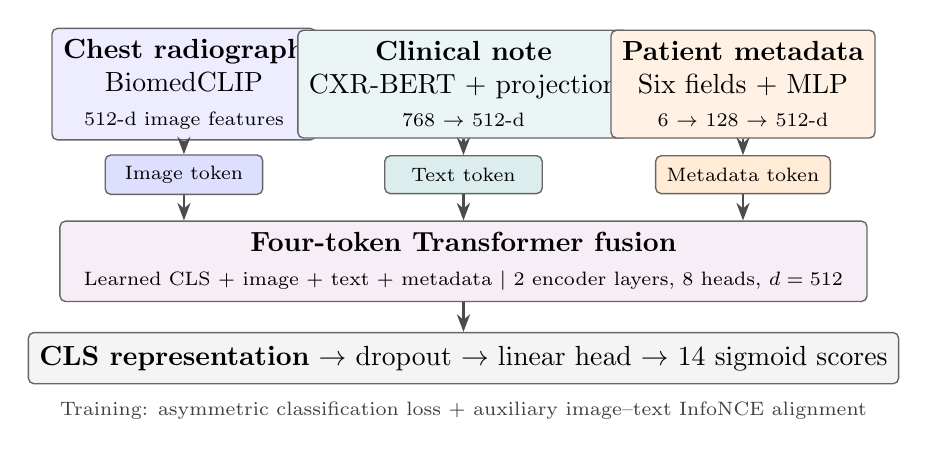
\begin{tikzpicture}[x=1cm,y=1cm,>=Stealth,
 box/.style={draw=black!60,rounded corners=2pt,line width=.5pt,align=center,inner sep=4pt},
 arrow/.style={->,line width=.75pt,draw=black!70},
 label/.style={font=\scriptsize,align=center}]
% Modality-specific encoders
\node[box,fill=blue!7,minimum width=3.15cm,minimum height=1.18cm] (vis) at (1.7,4.1)
 {\textbf{Chest radiograph}\\BiomedCLIP\\\scriptsize 512-d image features};
\node[box,fill=teal!8,minimum width=3.15cm,minimum height=1.18cm] (txt) at (5.25,4.1)
 {\textbf{Clinical note}\\CXR-BERT + projection\\\scriptsize 768 $\rightarrow$ 512-d};
\node[box,fill=orange!10,minimum width=3.15cm,minimum height=1.18cm] (met) at (8.8,4.1)
 {\textbf{Patient metadata}\\Six fields + MLP\\\scriptsize 6 $\rightarrow$ 128 $\rightarrow$ 512-d};
% tokens
\node[box,fill=blue!13,minimum width=2.0cm,minimum height=.48cm,font=\scriptsize] (vt) at (1.7,2.95) {Image token};
\node[box,fill=teal!14,minimum width=2.0cm,minimum height=.48cm,font=\scriptsize] (tt) at (5.25,2.95) {Text token};
\node[box,fill=orange!16,minimum width=2.0cm,minimum height=.48cm,font=\scriptsize] (mt) at (8.8,2.95) {Metadata token};
\draw[arrow] (vis.south)--(vt.north);\draw[arrow] (txt.south)--(tt.north);\draw[arrow] (met.south)--(mt.north);
% Fusion
\node[box,fill=violet!7,minimum width=10.25cm,minimum height=1.02cm] (fusion) at (5.25,1.85)
 {\textbf{Four-token Transformer fusion}\\\scriptsize Learned CLS + image + text + metadata $\mid$ 2 encoder layers, 8 heads, $d=512$};
\draw[arrow] (vt.south) -- (vt.south |- fusion.north);
\draw[arrow] (tt.south) -- (tt.south |- fusion.north);
\draw[arrow] (mt.south) -- (mt.south |- fusion.north);
\node[box,fill=gray!9,minimum width=7.1cm,minimum height=.65cm] (head) at (5.25,.62)
 {\textbf{CLS representation} $\rightarrow$ dropout $\rightarrow$ linear head $\rightarrow$ 14 sigmoid scores};
\draw[arrow] (fusion.south)--(head.north);
\node[label,text=black!75] at (5.25,-.05) {Training: asymmetric classification loss + auxiliary image--text InfoNCE alignment};
\end{tikzpicture}
}
\caption{X-Fusion architecture. Three encoders produce 512-dimensional modality tokens that join a learned CLS token in a two-layer Transformer. The classifier predicts fourteen finding scores. Visual attention and metadata-attribution displays are produced separately by the inference interface.}
\label{fig:architecture}
\end{figure}

\subsection{Optimization Objectives}

Let $p_{ik}$ be the predicted probability for finding $k$ in sample $i$, and $y_{ik}\in\{0,1\}$ its label. Define $q_{ik}=\min(1-p_{ik}+0.05,1)$. With $\epsilon=10^{-8}$, the per-label Asymmetric Loss term is

\begin{multline}
\ell_{ik}=
-y_{ik}(1-p_{ik})
\log(\max(p_{ik},\epsilon))\\
-(1-y_{ik})(1-q_{ik})^4
\log(\max(q_{ik},\epsilon)).
\end{multline}

The classification loss is $\mathcal{L}_{\mathrm{ASL}}=B^{-1}\sum_{i=1}^{B}\sum_{k=1}^{14}\ell_{ik}$. For normalized image and text features $v_i,t_j$, similarity is $C_{ij}=v_i^\top t_j/\tau$, where $\tau=0.07$. Symmetric contrastive alignment uses

\begin{align}
\mathcal{L}_{\mathrm{NCE}}
&=\tfrac{1}{2}
[\operatorname{CE}(C,a)+
\operatorname{CE}(C^\top,a)],\\
\mathcal{L}_{\mathrm{train}}
&=\mathcal{L}_{\mathrm{ASL}}
+0.1\mathcal{L}_{\mathrm{NCE}},
\end{align}

where $a$ contains matching image and text batch indices.

\section{Dataset and Experimental Setup}

\subsection{Data Partitioning}

The local study subset contains 31,630 images matched to metadata, drawn from 31,877 available PNG files. The full NIH release includes 112,120 radiographs \cite{nihdataset}. Training and validation images are selected from the official train and validation list, with patient IDs shuffled using seed 42 and 10\% of patients reserved for validation. Test images follow the official test list. The partitions contain no overlapping patient IDs.

Images are resized to $224\times224$ pixels, converted to RGB, and normalized using channel means $(0.485,0.456,0.406)$ and standard deviations $(0.229,0.224,0.225)$. Training augmentation includes horizontal flips, rotations up to $10^\circ$, and brightness and contrast jitter of 0.15. Validation and test preprocessing is deterministic. The fourteen findings are nonexclusive. ``No Finding'' is represented by an all-zero target vector.

\begin{table}[htbp]
\caption{Dataset partitions}
\label{tab:split}
\centering\small
\begin{tabular}{lrr}
\toprule
Partition & Images & Patients\\
\midrule
Training & 21,964 & 9,939\\
Validation & 2,566 & 1,104\\
Test & 7,100 & 1,137\\
\midrule
Total & 31,630 & 12,180\\
\bottomrule
\end{tabular}
\end{table}

\begin{table}[htbp]
\caption{Positive-label counts by partition}
\label{tab:prevalence}
\centering\small
\begin{tabular}{lrrr}
\toprule
Finding & Train & Validation & Test\\
\midrule
Atelectasis & 3237 & 367 & 879\\
Cardiomegaly & 723 & 107 & 387\\
Effusion & 2687 & 329 & 1270\\
Infiltration & 3629 & 433 & 1128\\
Mass & 1600 & 164 & 476\\
Nodule & 2111 & 226 & 476\\
Pneumonia & 42 & 5 & 18\\
Pneumothorax & 1148 & 131 & 1024\\
Consolidation & 132 & 11 & 62\\
Edema & 395 & 43 & 262\\
Emphysema & 557 & 70 & 335\\
Fibrosis & 558 & 57 & 190\\
Pleural Thickening & 787 & 94 & 348\\
Hernia & 63 & 8 & 49\\
\bottomrule
\end{tabular}
\end{table}

\subsection{Auxiliary Inputs and Training}

Age and sex come from image metadata. In the available experiment, clinical-note templates and sampled vital signs are conditioned on disease labels. This creates a dependency between auxiliary inputs and the target and is important when interpreting predictive metrics. Training uses AdamW, cosine annealing, a learning rate of $2\times10^{-4}$, weight decay of $10^{-4}$, batch size 4, gradient accumulation over eight batches, requested 16-bit mixed precision, and a frozen text encoder. The available checkpoint is from epoch 14 of a 15-epoch configuration.

\section{Artifact Reanalysis and Discussion}
\subsection{Optimization Records}
Fourteen logged epochs show the training objective decreasing from 0.1545 to 0.1190, a 22.95\% relative reduction, and validation ASL decreasing from 0.0207 to 0.0007. Training includes ASL and contrastive regularization, whereas validation records ASL alone. Their scales are not directly comparable. The traces document optimization of the configured objective, not independent diagnostic discrimination.
\begin{figure}[t]
\centering
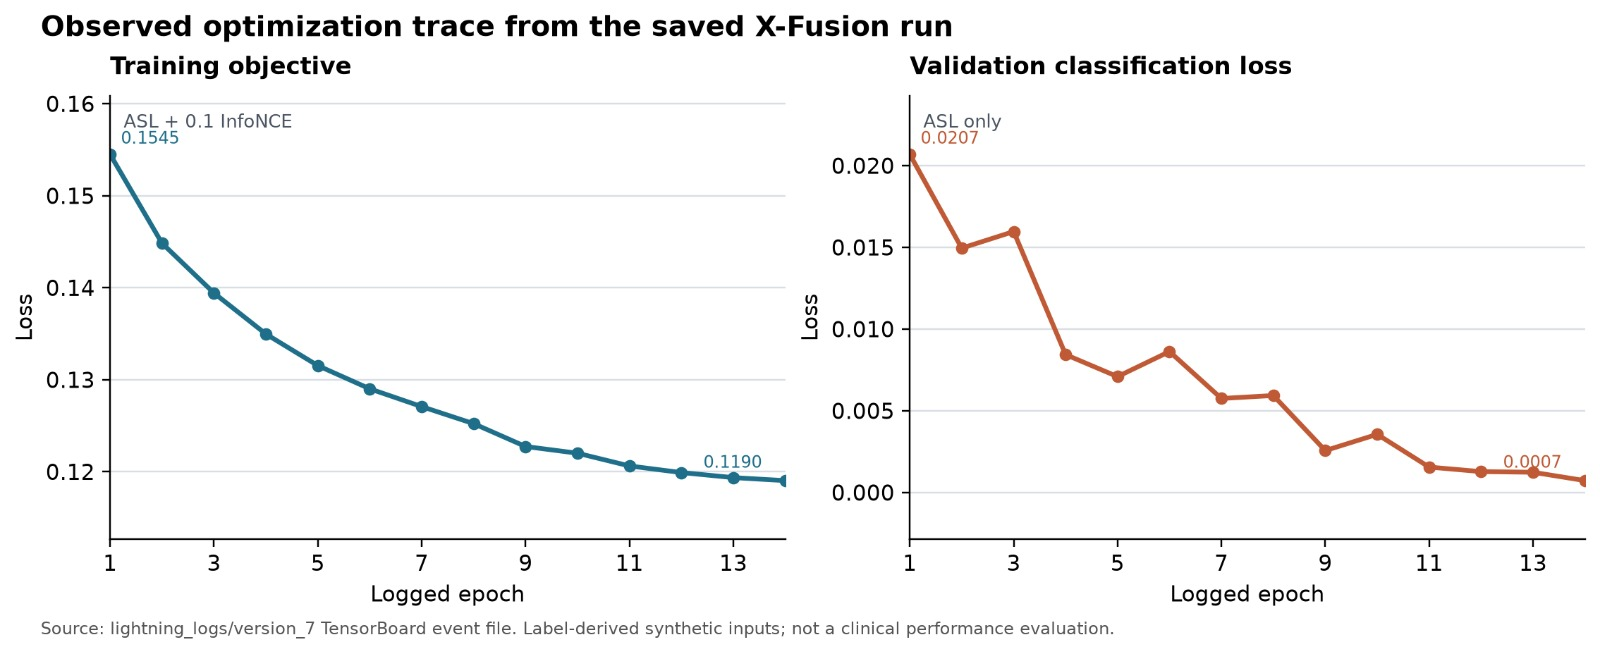
\includegraphics[width=\linewidth]{optimization_traces.jpg}
\caption{Saved optimization traces for fourteen epochs. Training and validation optimize different objectives; the auxiliary inputs are label-conditioned. The curves characterize optimization under the stated inputs.}
\label{fig:losses}
\end{figure}

\subsection{Recomputed Software Diagnostics}
The saved prediction file contains 7,100 distinct image identifiers, fourteen binary targets, and fourteen probability columns. We recomputed AUROC by grouping tied scores and integrating the empirical ROC curve, average precision by summing precision weighted by recall increments at distinct scores, and F1 from pooled per-label confusion counts at a fixed threshold of 0.5. Macro scores are unweighted means over fourteen findings. Average precision is reported explicitly; it is not assumed identical to trapezoidal area under a precision--recall curve. This analysis reuses saved outputs and does not rerun inference or establish their full generation history.

\begin{table}[t]
\caption{\textbf{Label-conditioned pipeline diagnostics---not clinical validation.} Target-derived notes and vital signs were available at evaluation; these values must not be compared with independent-input clinical benchmarks.}
\label{tab:diagnostics}
\centering
\begin{tabular}{lr}
\toprule
Quantity & Diagnostic value\\
\midrule
Macro AUROC & 0.999961\\
Macro average precision & 0.995327\\
Macro F1 at 0.5 & 0.970857\\
Pneumonia precision at 0.5 & 0.566667\\
Pneumonia recall at 0.5 & 0.944444\\
Pneumonia F1 at 0.5 & 0.708333\\
\bottomrule
\end{tabular}
\end{table}

The near-perfect macro ranking scores must be interpreted in the context of input construction. The generator builds notes from disease labels and samples four physiological fields conditional on Pneumonia or Edema. Thus, target information is present in predictors for test cases. Patient-disjoint image lists address patient overlap but cannot break this within-case dependency. No improvement over image-only prediction can be attributed to independently observed clinical information from these results.

For Pneumonia, the saved predictions yield 17 true positives, 13 false positives, and one false negative at 0.5, among 18 positive and 7,082 negative cases. This explains how high aggregate ranking scores can coexist with modest precision on a rare label. The threshold is used for descriptive reproduction only and is not selected or recommended from test outcomes. The 18 positive Pneumonia images come from only 12 patients. One image changes pooled recall by $1/18$ (5.56 percentage points). Image-level binomial intervals would ignore within-patient dependence; the independent-baseline uncertainty analysis below therefore resamples patients. Sparse positives still limit the stability of rare-label estimates.

Earlier aggregate comparisons and modality ablations lack matching prediction-level artifacts for their configurations. They are excluded from this analysis. Without matched tri-modal baselines, controlled fusion ablations, statistical uncertainty estimates, and independently collected auxiliary inputs, the original evidence supports an implementation description and a leakage diagnosis rather than a claim of diagnostic superiority. The separate reference experiment below supplies narrower comparative evidence.

\subsection{Independent-Input Reference Experiment}
We trained new reference models using the same patient-disjoint image lists, without the generated notes, synthetic vital signs, or the X-Fusion checkpoint. The four configurations are training-label prevalence, recorded age and sex, image pixels, and image pixels plus recorded age and sex. The prevalence predictor is constant for each label and uses training targets only. All other models fit fourteen independent L2-regularized logistic regressions. These deliberately simple models provide reproducible reference evidence; they are not substitutes for pretrained image encoders or an ablation of the tri-modal Transformer.

Images are converted to grayscale and bilinearly resized to $16\times16$, producing 256 pixel predictors scaled to $[0,1]$. Age values outside $[0,120]$ or missing are replaced with the training-partition median. The recorded binary gender field is encoded as M=1 and F=0, with missing values set to 0.5. All predictor standardization is fitted on training cases only. No predictor is generated from a finding label. The image and combined models share identical pixel features and eligible cases.

For each configuration, regularization strength $C\in\{0.01,0.1,1\}$ is selected by validation macro AUROC. We use the L-BFGS solver, at most 500 iterations, and seed 42; all selected label models converge before the iteration limit. The selected models are evaluated on the test partition after validation selection. Thresholded F1 uses a fixed 0.5 cutoff rather than a test-selected threshold. Table~\ref{tab:independent} reports the resulting held-out reference scores.

\begin{table}[t]
\caption{New independent-input reference experiment on 7,100 test-list images. These scores are separate from the contaminated X-Fusion diagnostics and do not validate tri-modal fusion. AP denotes average precision; F1 uses threshold 0.5.}
\label{tab:independent}
\centering\small
\begin{tabular}{lrrr}
\toprule
Configuration & Macro AUROC & Macro AP & Macro F1\\
\midrule
Training prevalence & 0.5000 & 0.0695 & 0.0000\\
Recorded age and sex & 0.5518 & 0.0861 & 0.0000\\
Image pixels & 0.6317 & 0.1178 & 0.0098\\
Image pixels + age and sex & 0.6344 & 0.1201 & 0.0106\\
\bottomrule
\end{tabular}
\end{table}

Validation selects age/sex $C=0.1$, pixels $C=0.01$, pixels plus age/sex $C=0.01$. Numerical differences describe these linear reference models; they do not establish a benefit of clinical notes, vital signs, pretrained encoders, or Transformer fusion. A comparison between these models and the contaminated X-Fusion scores would change both the predictors and model family and is not a valid estimate of a fusion effect.

The experiment archives its executable script, exact patient partitions, selected hyperparameters, aggregate and per-label metrics, and per-case test targets and probabilities. It tests a narrower image-and-demographics task with independent predictors. Independent clinical context and retraining of the tri-modal architecture remain necessary for the original clinical-generalization claim.

\begin{figure}[t]
\centering
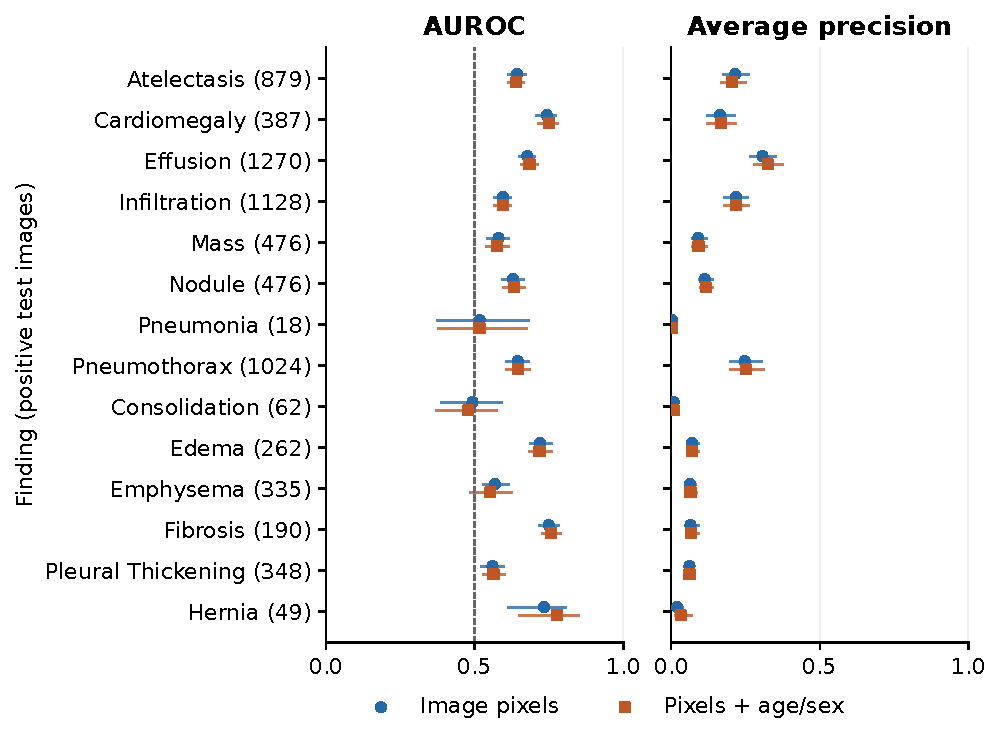
\includegraphics[width=\linewidth]{per_disease_performance.pdf}
\caption{Per-disease performance recomputed from genuine saved predictions of the independent-input linear baselines. Parentheses give positive test-image counts. Horizontal lines are exploratory 95\% patient-cluster bootstrap intervals (500 resamples); points are the original test estimates. The dashed AUROC line marks 0.5. These are not X-Fusion results.}
\label{fig:disease}
\end{figure}

Figure~\ref{fig:disease} shows disease-level AUROC and average precision rather than aggregate scores alone. We resampled the 1,137 test patients with replacement 500 times (seed 20261015), retaining all images for each sampled patient with its sampling multiplicity. Models and thresholds remain fixed; these exploratory percentile intervals describe test-sample uncertainty conditional on the fitted models, not uncertainty from training or hyperparameter selection. Replicates lacking either class for a finding are excluded for that finding; valid counts are archived. Rare-label intervals remain unstable when few positive patients are available.

The paired macro AUROC difference for pixels plus age/sex minus pixels is 0.0027, with a 95\% patient-cluster bootstrap interval of [-0.0019, 0.0070]. The interval includes zero; this experiment does not establish a reliable improvement from demographics.

\subsection{Explanation Views and Application Behavior}
The interface averages CLS-to-patch attention across the twelve heads in the final block of the BiomedCLIP ViT-B/16 visual backbone, arranges weights on a $14\times14$ patch grid, and overlays them on the image. These twelve visual-backbone heads are distinct from the eight heads in each multimodal fusion encoder layer. The overlay is extracted before fusion and does not visualize fusion attention. This is an attention display, not Chefer relevance propagation or validated lesion localization. It is not finding-specific causal evidence. Kernel SHAP perturbs the six metadata fields while image and text features remain fixed. Absolute contributions are aggregated across fourteen outputs and normalized. Aggregation removes the sign and finding specificity of contributions; an all-zero background can represent implausible physiological combinations.

A Next.js frontend communicates with a FastAPI inference service. The interface accepts a radiograph, clinical text, and six structured fields and returns finding scores with separate explanation views. Missing fields use configured defaults, and a leading score of 0.30 controls the displayed finding status. These choices implement a demonstration workflow. They have not been clinically calibrated or validated as a missing-data strategy. No user study, prospective deployment outcome, or clinical utility claim is made.

\section{Evaluation Scope and Next Steps}
The label-conditioned tri-modal diagnostics cannot estimate clinical accuracy. The independent-input models address a narrower task, use very low-resolution image features, and do not measure the actual X-Fusion architecture. No leakage-free BiomedCLIP versus X-Fusion comparison has been completed. The data contain no independently acquired clinical notes or vital signs, so the original tri-modal benefit claim remains unsupported.

A matched next experiment should train an image-only BiomedCLIP head and a reduced fusion model using the same image embeddings and recorded age/sex, with identical patient splits, preprocessing, optimization budgets, and validation-based selection. This would test image--demographic fusion, not tri-modal clinical fusion. Simply masking inputs in the contaminated checkpoint would test distribution shift rather than repair its training. A valid tri-modal experiment additionally requires independently observed clinical inputs available at prediction time, and new training from an uncontaminated initialization. External evaluation, calibration, and quantitative explanation benchmarks remain necessary before clinical claims.

\section{Conclusion}
X-Fusion implements a compact integration of pretrained visual and language encoders, structured attributes, and separate explanation views. New patient-disjoint linear reference experiments and disease-level uncertainty analysis provide reproducible evidence for a narrower image-and-demographics task. Their small aggregate difference does not establish demographic benefit, and the original label-conditioned scores do not validate tri-modal fusion. Assessing X-Fusion requires matched encoder and fusion experiments with independently observed inputs.

\bibliographystyle{splncs04}
\bibliography{references}
\end{document}
